\newpage
\section{Interpretability}
\label{sec:results_interpretability}
The results from the experiments, as described in \autoref{sec:interpretabilityoftools}, will be shown in this section, to answer the fourth research question: \textit{Do these data profiles provide more interpretability of error detection tools?}

\subsection{Feature selection}
\label{subsec:interpretability_results_feature_selection}
% Permutation importance feature selection
To improve machine learning models, dimensionality reduction can be a solution. Permutation importance was calculated for all the features of the dataset profiles for the best performing strategies, after all the estimators were trained. All the features that had a positive impact on the model prediction outcome were kept. 46 out of the original 72 features were kept. Now, using this hindsight information, the models were retrained with only those features. To compare the two sets of features used, the mean squared error (MSE) and median absolute error (MAE) are shown in \autoref{tab:improvements_feature_selection}. It shows that the improvements are negligible.

\begin{table}[h]
\centering
\begin{tabular}{l|ll|ll}
\textbf{Metric} & \textbf{MSE 1} & \textbf{MAE 1} & \textbf{MSE 2} & \textbf{MAE 2} \\ \hline
Precision       & 0.0543         & 0.0949         & \textbf{0.0532}         & \textbf{0.0948}         \\
Recall          & \textbf{0.1045}         & 0.166          & 0.1048         & \textbf{0.1578}         \\
Direct F1       & 0.0442         & \textbf{0.1006}         & \textbf{0.0440}         & 0.1007         \\
Combined F1     & \textbf{0.0452}         & 0.0790         & 0.0455         & \textbf{0.0775}        
\end{tabular}
\caption{Estimation score comparison - 1 all features / 2 reduced number of features (best scores in bold)}
\label{tab:improvements_feature_selection}
\end{table}


\subsection{Feature importance}
The feature importance of the dataset profile features will be analyzed using SHAP values of the estimators produced in \autoref{sec:performanceprediction}. The first part below will be contributed to a general overview of feature importance for all direct F1 estimator models. Then, from the second subsection, a more detailed precision and recall feature importance analysis will be conducted for every error detection tool.

\subsubsection{General F1-score analysis}
For every best scoring strategy per tool, the feature importance analysis of the direct F1-estimator was done. The extensive results can be found in \autoref{appsec:f1_feature_importance}. For FAHES \& Forbidden Itemsets, no feature importance could be extracted using the direct F1 estimator.
For every other tool, The key takeaways were that an increase in $cells\_length\_variance$ and/or  $characters\_alphabet\_variance$ would have a negative impact on the performance (F1).
This can be attributed to the fact that, whenever lengths of cells and the number of alphabetical characters vary across columns, the data is less structured. Less structured data seems harder to detect errors in. While these two features are most important for the direct F1 estimations of all error detection tools, the model output still varies for each tool. A less structured dataset will have a different relative impact for each tool, but it is still a common issue for all datasets.

% ---------------------------------------------
% ---------------------------------------------
% ---------------------------------------------
% ---------------------------------------------
% ---------------------------------------------
% ---------------------------------------------

\subsubsection{ActiveClean}
\label{subsubsec:importance_ActiveClean}
To start the detailed review, ActiveClean will be discussed first. The first step in the feature performance analysis was to find the top influential features of the dataset profile to estimate the performance of the tool. In \autoref{fig:feature_importance_prec_ActiveClean}, the ten most influential features for precision are shown and in \autoref{fig:feature_importance_rec_ActiveClean} for recall. 

\begin{figure}[H]
    \centering
    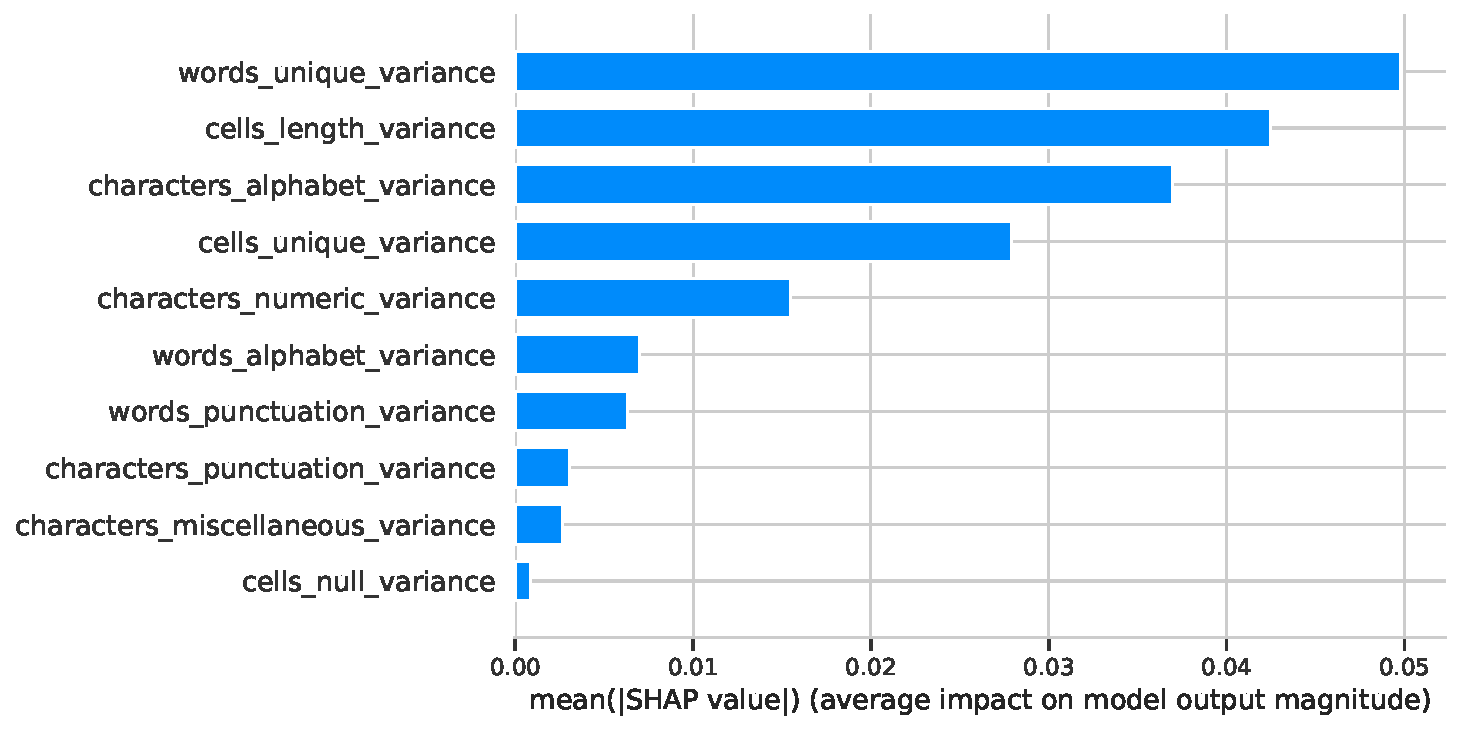
\includegraphics[width=0.9\textwidth]{thesis/Figures/RQ4/Shap_cell_prec_ActiveClean.pdf}
    \caption{ActiveClean - Top 10 Precision influential features according to SHAP values}
    \label{fig:feature_importance_prec_ActiveClean}
\end{figure}
\begin{figure}[H]
    \centering
    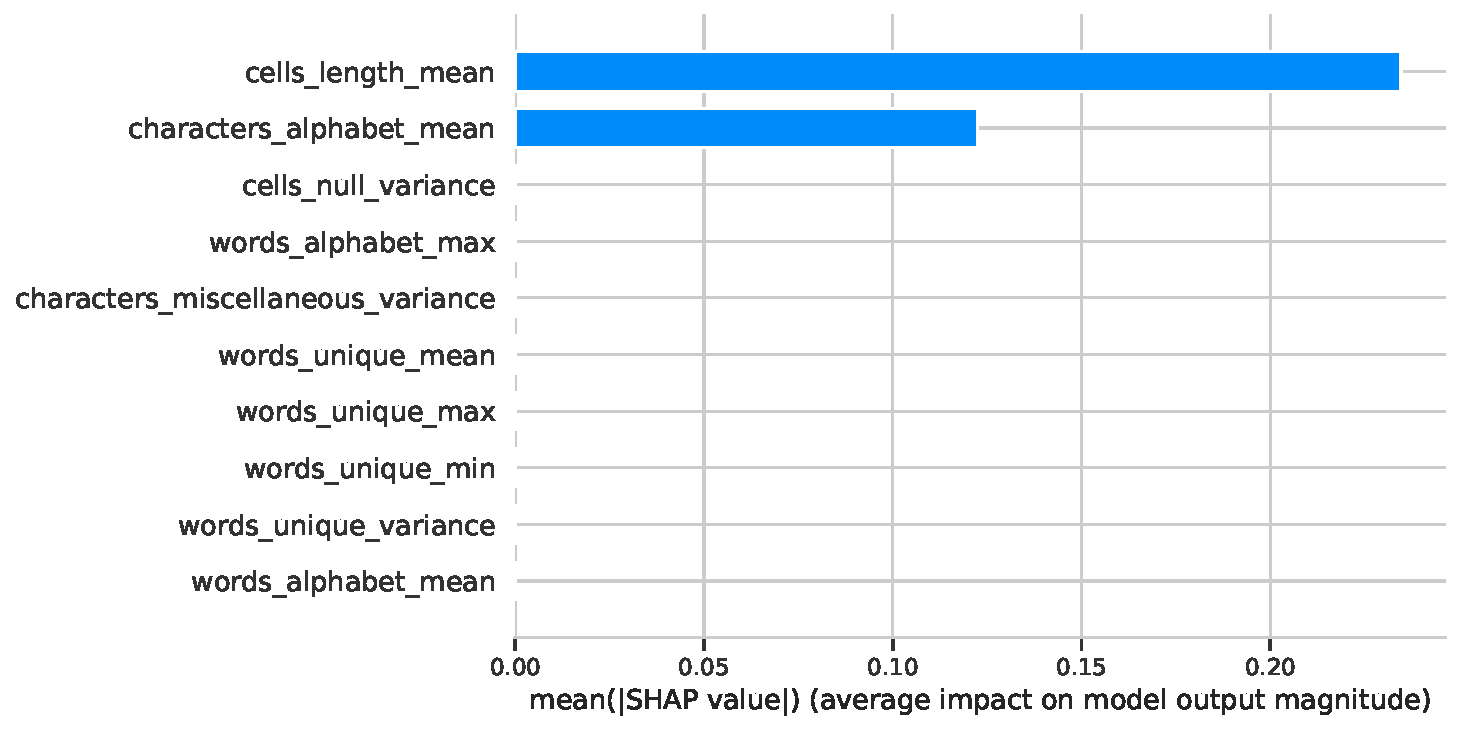
\includegraphics[width=0.9\textwidth]{thesis/Figures/RQ4/Shap_cell_rec_ActiveClean.pdf}
    \caption{ActiveClean - Top 10 Recall influential features according to SHAP values}
    \label{fig:feature_importance_rec_ActiveClean}
\end{figure}

The figures above give a clear indication on the average impact on the model outputs. It shows that for the precision estimation, all top 10 features have impact on the model output. However, for the recall estimation, only 2 features are found to be beneficial for estimation.
~\\The next step in the analysis for extract interpretability was trying to correlate the input features to the relative contribution they make on the model output. Then, these correlations need to be translated into logic or relations between the dataset profiles and the functioning of an error detection tool.


\begin{table}[H]
	\centering
	\addtolength{\leftskip} {-2cm}
	\addtolength{\rightskip}{-2cm}
	\captionsetup[subtable]{position = below}
	\captionsetup[table]{position=top}
	\caption{Top feature influences - ActiveClean}
	\label{tab:feature_influences_ActiveClean}
		\begin{subtable}{0.5\linewidth}
		\centering
		\begin{tabular}{llr}
\toprule
 \# &                         Feature &         Influence \\
\midrule
 1 &         words\_unique\_variance &   0.39 $\nearrow$ \\
 2 &         cells\_length\_variance &  -0.42 $\searrow$ \\
 3 &  characters\_alphabet\_variance &  -0.39 $\searrow$ \\
\bottomrule
\end{tabular}
		\caption{Precision feature influences - ActiveClean}
		\label{tab:prec_feature_influences_ActiveClean}
	\end{subtable}
	\hspace*{4em}
	\begin{subtable}{0.5\linewidth}
		\centering
		\begin{tabular}{llr}
\toprule
 \# &                     Feature &         Influence \\
\midrule
 1 &         cells\_length\_mean &  -0.09 $\searrow$ \\
 2 &  characters\_alphabet\_mean &  -0.12 $\searrow$ \\
 3 &       - &                 - \\
\bottomrule
\end{tabular}
		\caption{Recall feature influences - ActiveClean}
		\label{tab:rec_feature_influences_ActiveClean}
	\end{subtable}%
\end{table}

In \autoref{tab:prec_feature_influences_ActiveClean}, the correlations/influences of the three most impactful features are shown for precision. It shows that a higher $words\_unique\_variance$ will have a positive impact on the prediction and $cells\_length\_variance$ as well as \\$characters\_alphabet\_variance$ have a negative influence with higher values. The positive impact of the variance of the number of unique words across columns can be attributed to the fact that ActiveClean makes use of the frequency of (co-)occurrences of words, so having more unique words in some columns and more similar words in other columns, makes rows distinguishable to find duplicates or rule violations. Having higher $cells\_length\_variance$ and $characters\_alphabet\_variance$ will manifest as unstructured data with varying character types across columns, which has a negative impact on ActiveClean.
In \autoref{tab:rec_feature_influences_ActiveClean}, the influences of the most important features for recall are shown. Because only 2 features had an impact, only two will be discussed. The average length of cells and the average number of alphabetical characters per column negatively impact the model output. This could be attributed to the fact that datasets with large values and only alphabetical values will be indistinguishable for ActiveClean. This results in marking each value as erroneous, which will lead to a higher recall. 

% ---------------------------------------------
% ---------------------------------------------
% ---------------------------------------------
% ---------------------------------------------
% ---------------------------------------------
% ---------------------------------------------


\subsubsection{dBoost}
\label{subsubsec:importance_dBoost}
For dBoost and the following tools in this chapter, only the correlation tables will be shown. The full impact bar plots for the top 10 influential features can be found in \autoref{appsec:prec_rec_feature_importance} of the appendix. Also, more condensed explanations for the feature importance will be given, as the main thinking pattern was shown in the section above. 

\begin{table}[H]
	\centering
	\addtolength{\leftskip} {-2cm}
	\addtolength{\rightskip}{-2cm}
	\captionsetup[subtable]{position = below}
	\captionsetup[table]{position=top}
	\caption{Top feature influences - dBoost}
	\label{tab:feature_influences_dBoost}
		\begin{subtable}{0.5\linewidth}
		\centering
		\begin{tabular}{llr}
\toprule
 \# &                         Feature &         Influence \\
\midrule
 1 &         cells\_length\_variance &  -0.79 $\searrow$ \\
 2 &  characters\_alphabet\_variance &  -0.59 $\searrow$ \\
 3 &         cells\_unique\_variance &   0.72 $\nearrow$ \\
\bottomrule
\end{tabular}
		\caption{Precision feature influences - dBoost}
		\label{tab:prec_feature_influences_dBoost}
	\end{subtable}
	\hspace*{4em}
	\begin{subtable}{0.5\linewidth}
		\centering
		\begin{tabular}{llr}
\toprule
 \# &                       Feature &         Influence \\
\midrule
 1 &  cells\_punctuation\_variance &  -0.39 $\searrow$ \\
 2 &              cells\_null\_max &   0.29 $\nearrow$ \\
 3 &         - &                 - \\
\bottomrule
\end{tabular}
		\caption{Recall feature influences - dBoost}
		\label{tab:rec_feature_influences_dBoost}
	\end{subtable}%
\end{table}

As seen in \autoref{tab:prec_feature_influences_dBoost}, for the precision feature importance, the two most impactful features are the same as the general F1 feature importance analysis. dBoost is negatively impacted in terms of precision if the dataset is less structured (varying cell lengths and varying character types). Being based on multivariate outliers for detecting errors, the third feature $cells\_unique\_variance$ can positively influence the results if higher. A variance across columns for unique cells makes it such that columns can have identifying values in one column (low number of unique cells), like a category, and then outliers of a certain rule (high number of unique cells) in another column, making errors identifiable. 
And as seen in \autoref{tab:rec_feature_influences_dBoost}, the recall is negatively impacted if, across columns, the cells containing punctuation vary, which might be attributed to the inability to find appropriate expansion schemes for these cells. If there are many null cells in the dataset, the recall improves, as they are common errors and detectable by dBoost.

% ---------------------------------------------
% ---------------------------------------------
% ---------------------------------------------
% ---------------------------------------------
% ---------------------------------------------
% ---------------------------------------------

\subsubsection{FAHES}
As can be seen in \autoref{tab:prec_feature_influences_FAHES}, precision for FAHES is positively impacted by varying unique cells across columns, which could make errors more identifiable. Furthermore, it is negatively impacted by unstructured data ($cells\_length\_variance$ and $characters\_alphabet\_variance$). However, if the cells in the data are varying of type (alphabetic or numeric), across columns, the recall improves (\autoref{tab:rec_feature_influences_FAHES}).

\begin{table}[H]
	\centering
	\addtolength{\leftskip} {-2cm}
	\addtolength{\rightskip}{-2cm}
	\captionsetup[subtable]{position = below}
	\captionsetup[table]{position=top}
	\caption{Top feature influences - FAHES}
	\label{tab:feature_influences_FAHES}
		\begin{subtable}{0.5\linewidth}
		\centering
		\begin{tabular}{llr}
\toprule
 \# &                         Feature &         Influence \\
\midrule
 1 &         cells\_unique\_variance &   0.67 $\nearrow$ \\
 2 &         cells\_length\_variance &  -0.59 $\searrow$ \\
 3 &  characters\_alphabet\_variance &  -0.59 $\searrow$ \\
\bottomrule
\end{tabular}
		\caption{Precision feature influences - FAHES}
		\label{tab:prec_feature_influences_FAHES}
	\end{subtable}
	\hspace*{4em}
	\begin{subtable}{0.5\linewidth}
		\centering
		\begin{tabular}{llr}
\toprule
 \# &                    Feature &        Influence \\
\midrule
 1 &  cells\_alphabet\_variance &  0.66 $\nearrow$ \\
 2 &   cells\_numeric\_variance &  0.61 $\nearrow$ \\
 3 &      - &                - \\
\bottomrule
\end{tabular}
		\caption{Recall feature influences - FAHES}
		\label{tab:rec_feature_influences_FAHES}
	\end{subtable}%
\end{table}

% ---------------------------------------------
% ---------------------------------------------
% ---------------------------------------------
% ---------------------------------------------
% ---------------------------------------------
% ---------------------------------------------


\subsubsection{Forbidden Itemsets}
For Forbidden Itemsets, the most influential features are shown in \autoref{tab:prec_feature_influences_ForbiddenItemsets} and \autoref{tab:rec_feature_influences_ForbiddenItemsets}, for precision and recall, respectively. If the length of the cells varies across columns, precision improves. Forbidden Itemsets works with identifying "unlikely" value pairs, so if errors have other lengths than non-errors, this could make them detectable by the tool. It is not straightforward to interpret the impact of the unique cells and words on precision, as there is no clear correlation between the features and the impact. This shows that there is not a simple correlation to explain the impact.
Also, recall improves if the datasets contain larger words and more varying words.

\begin{table}[H]
	\centering
	\addtolength{\leftskip} {-2cm}
	\addtolength{\rightskip}{-2cm}
	\captionsetup[subtable]{position = below}
	\captionsetup[table]{position=top}
	\caption{Top feature influences - Forbidden Itemsets}
	\label{tab:feature_influences_ForbiddenItemsets}
		\begin{subtable}{0.5\linewidth}
		\centering
\begin{tabular}{llr}
\toprule
 \# &                  Feature &          Influence \\
\midrule
 1 &  cells\_length\_variance &    0.36 $\nearrow$ \\
 2 &  cells\_unique\_variance &  0.0 $\rightarrow$ \\
 3 &  words\_unique\_variance &   -0.18 $\searrow$ \\
\bottomrule
\end{tabular}
		\caption{Precision feature influences - Forbidden Itemsets}
		\label{tab:prec_feature_influences_ForbiddenItemsets}
	\end{subtable}
	\hspace*{4em}
	\begin{subtable}{0.5\linewidth}
		\centering
\begin{tabular}{llr}
\toprule
 \# &                  Feature &        Influence \\
\midrule
 1 &  words\_length\_variance &   0.3 $\nearrow$ \\
 2 &       words\_length\_min &  0.23 $\nearrow$ \\
 3 &     - &                - \\
\bottomrule
\end{tabular}
		\caption{Recall feature influences - Forbidden Itemsets}
		\label{tab:rec_feature_influences_ForbiddenItemsets}
	\end{subtable}%
\end{table}

% ---------------------------------------------
% ---------------------------------------------
% ---------------------------------------------
% ---------------------------------------------
% ---------------------------------------------
% ---------------------------------------------


\subsubsection{KATARA}
For KATARA the feature importance for the three most impactful features are shown in \autoref{tab:prec_feature_influences_KATARA} and \autoref{tab:rec_feature_influences_KATARA}. The three features that impact precision show that it needs structured cells, mostly alphabetical characters and words, in order to achieve higher precision. This seems logical, as KATARA is solely based on relations in knowledge bases based on known words. The recall is mostly slightly negatively influenced by the number of average punctuation characters and miscellaneous words, as these are not present in the knowledge base powering KATARA.

\begin{table}[H]
	\centering
	\addtolength{\leftskip} {-2cm}
	\addtolength{\rightskip}{-2cm}
	\captionsetup[subtable]{position = below}
	\captionsetup[table]{position=top}
	\caption{Top feature influences - KATARA}
	\label{tab:feature_influences_KATARA}
		\begin{subtable}{0.5\linewidth}
		\centering
\begin{tabular}{llr}
\toprule
 \# &                         Feature &        Influence \\
\midrule
 1 &       words\_alphabet\_variance &  0.29 $\nearrow$ \\
 2 &         cells\_length\_variance &  -0.2 $\searrow$ \\
 3 &  characters\_alphabet\_variance &  0.11 $\nearrow$ \\
\bottomrule
\end{tabular}

		\caption{Precision feature influences - KATARA}
		\label{tab:prec_feature_influences_KATARA}
	\end{subtable}
	\hspace*{4em}
	\begin{subtable}{0.5\linewidth}
		\centering
\begin{tabular}{llr}
\toprule
 \# &                        Feature &            Influence \\
\midrule
 1 &  characters\_punctuation\_mean &  -0.05 $\rightarrow$ \\
 2 &     words\_miscellaneous\_mean &     -0.07 $\searrow$ \\
 3 &            - &      - \\
\bottomrule
\end{tabular}
		\caption{Recall feature influences - KATARA}
		\label{tab:rec_feature_influences_KATARA}
	\end{subtable}%
\end{table}

% ---------------------------------------------
% ---------------------------------------------
% ---------------------------------------------
% ---------------------------------------------
% ---------------------------------------------
% ---------------------------------------------


\subsubsection{Raha}
Lastly, the feature importance for Raha is shown in \autoref{tab:prec_feature_influences_Raha} and \autoref{tab:rec_feature_influences_Raha}.
Raha's precision is negatively impacted by the number of miscellaneous characters and unstructured columns (varying cell length). The recall estimation is not impacted by any of the input features from the data profile. The estimator will most likely have a single recall value as output, meaning that it was not capable of learning from the dataset profiles with regards to the recall of Raha. 

\begin{table}[H]
	\centering
	\addtolength{\leftskip} {-4cm}
	\addtolength{\rightskip}{-4cm}
	\captionsetup[subtable]{position = below}
	\captionsetup[table]{position=top}
	\caption{Top feature influences - Raha}
	\label{tab:feature_influences_Raha}
		\begin{subtable}{0.5\linewidth}
		\centering
		\begin{tabular}{llr}
\toprule
 \# &                              Feature &         Influence \\
\midrule
 1 &      characters\_miscellaneous\_mean &  -0.42 $\searrow$ \\
 2 &  characters\_miscellaneous\_variance &  -0.35 $\searrow$ \\
 3 &              cells\_length\_variance &   -0.2 $\searrow$ \\
\bottomrule
\end{tabular}
		\caption{Precision feature influences - Raha}
		\label{tab:prec_feature_influences_Raha}
	\end{subtable}
	\hspace*{4em}
	\begin{subtable}{0.5\linewidth}
		\centering
\begin{tabular}{llr}
\toprule
 \# &                              Feature & Influence \\
\midrule
 1 &                - &         - \\
 2 &                     - &         - \\
 3 &  - &         - \\
\bottomrule
\end{tabular}
		\caption{Recall feature influences - Raha}
		\label{tab:rec_feature_influences_Raha}
	\end{subtable}%
\end{table}

\subsection{Evaluation}

% % The feature selection results produced from repeating the experiments from Section
% 4.2 will be compared on the mean squared error and mean absolute error to
% check for improvements.
To see if interpretability in retrospect would help improve the estimator models using feature selection, the estimator models were tested with the regular dataset profiles input and the reduced feature set dataset profiles in \autoref{subsec:interpretability_results_feature_selection}. No clear improvement has been made in automating the feature selection in retrospect. Different selection criteria could yield different results, but that could be looked into in future work. 

% The top features have a strong impact on the estimator model output
% The correlations are translatable to theories or logic about the features impact
% on the model output

As stated in the methodology, the main focus laid on whether the dataset profiles and estimators for the best performing configurations per tool would provide interpretability. In general (found by the F1 estimator feature importances), it was found that error detection tools benefit from structured data, with less variance between the length and content (characters) of cells. 
For the precision feature importance, it was possible to identify at least three features, for every tool, that had a strong impact on the model output and could give an estimated explanation of how and when the tool would work properly.
However, for recall, it was not possible to identify multiple impactful features and for some tools even no features. 

Besides finding impactful features, it was tested if the impactful features could be correlated with impact to translate the findings to theories or logic about the characteristics of a dataset. An attempt at giving logical explanations was provided in the previous sections. But, it was not tested in this research whether these findings hold for every situation. It was not possible for every impactful feature to find a strong correlation with respect to the output. However, for the majority of the tools, a link between a dataset characteristic (dataset profile feature) and the influence on a performance score could be made. 

% Mostly using ranking
Adding interpretability using SHAP values is only possible for a single estimator at a time. It would not be feasible to integrate SHAP analysis in the strategy ranking system, but it could be used to give confidence to a suggestion when a final error detection strategy has already been selected. Further analysis could be done on explaining the predictions of performance scores for a single dataset and error detection strategy at one time in more detail. This would possibly give more confidence in the suggestions to the experts using the predictions and suggested rankings made by the system proposed in this research. 

~\\Considering the evaluation from above, it has been shown that it is possible to provide some insights on the performance of error detection tools using interpretability methods with regards to features from the dataset profiles. However, work needs to be done in order to integrate the interpretability methods in an error detection workflow and verify the produced results and logic from the SHAP values. But concluding, it can be deemed true that the data profiles provide more interpretability of error detection tools. 